\documentclass[border=4pt]{standalone}
\usepackage{mathptmx,tikz}
\usetikzlibrary{arrows.meta,calc}
\definecolor{velocity}{HTML}{1F77B4}
\definecolor{force}{HTML}{D62728}
\begin{document}
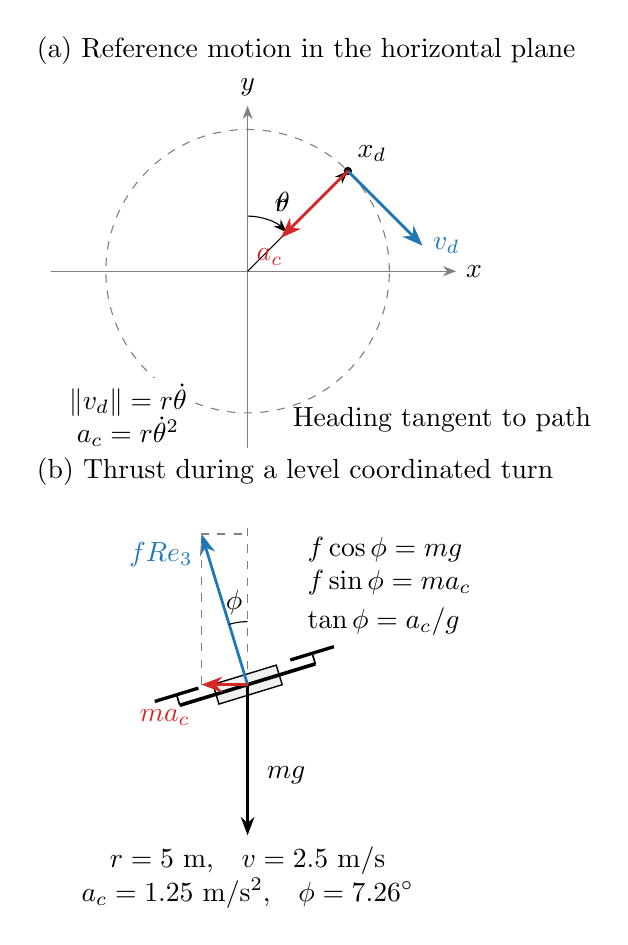
\begin{tikzpicture}[>=Stealth,font=\fontsize{10}{12}\selectfont]
\node[anchor=west] at (-2.8,2.8) {(a) Reference motion in the horizontal plane};
\draw[->,gray] (-2.5,0)--(2.65,0) node[right,black] {$x$};
\draw[->,gray] (0,-2.25)--(0,2.10) node[above,black] {$y$};
\draw[gray,dashed] (0,0) circle[radius=1.8];
\coordinate (P) at (1.273,1.273);
\draw[->,black] (0,0)--(P) node[midway,above left] {$r$};
\draw[->] (0,0.7) arc[start angle=90,end angle=45,radius=.7];
\node at (.45,.88) {$\theta$};
\fill (P) circle[radius=1.5pt];
\node[above right] at (P) {$x_d$};
\draw[->,velocity,line width=1pt] (P)--++(.95,-.95)
 node[right,text=velocity] {$v_d$};
\draw[->,force,line width=1pt] (P)--++(-.85,-.85);
\node[text=force] at (.28,.18) {$a_c$};
\node[align=center,fill=white,inner sep=2pt] at (-1.52,-1.83)
 {$\|v_d\|=r\dot\theta$\\$a_c=r\dot\theta^2$};
\node[anchor=west] at (.45,-1.88) {Heading tangent to path};
\begin{scope}[yshift=-5.25cm]
\node[anchor=west] at (-2.8,2.70) {(b) Thrust during a level coordinated turn};
\draw[dashed,gray] (0,-1.7)--(0,2);
\begin{scope}[rotate=17]
  \draw[fill=gray!12,draw=black,line width=.5pt] (-.42,-.13) rectangle (.42,.13);
  \draw[line width=1.3pt] (-.9,0)--(.9,0);
  \draw[line width=.6pt] (-.9,0)--(-.9,.14) (.9,0)--(.9,.14);
  \draw[line width=1.2pt] (-1.19,.14)--(-.61,.14) (.61,.14)--(1.19,.14);
\end{scope}
\draw[->,velocity,line width=1pt] (0,0)--(-.585,1.913);
\node[text=velocity] at (-1.1,1.65) {$fRe_3$};
\draw[->,black,line width=.8pt] (0,0)--(0,-1.913);
\node[anchor=west] at (.12,-1.15) {$mg$};
\draw[->,force,line width=1pt] (0,0)--(-.585,0);
\node[text=force,fill=white,inner sep=1pt] at (-1.05,-.42) {$ma_c$};
\draw[dashed,gray] (-.585,0)--(-.585,1.913)--(0,1.913);
\draw (0,.8) arc[start angle=90,end angle=107,radius=.8];
\node at (-.17,1.04) {$\phi$};
\node[anchor=west,align=left,fill=white,inner sep=3pt] at (.65,1.25)
 {$f\cos\phi=mg$\\$f\sin\phi=ma_c$\\[2pt]$\tan\phi=a_c/g$};
\node[align=center] at (0,-2.45) {$r=5$ m,\quad $v=2.5$ m/s\\$a_c=1.25$ m/s$^2$,\quad $\phi=7.26^\circ$};
\end{scope}
\end{tikzpicture}
\end{document}
